\chapter{Results and Evaluation} This chapter includes a comparison and analysis of results generated by the text encapsulation toolkit(here onwards referred to as 
TET). The auto generated extracts(one third of the document length) of fifty randomly selected news articles from test data, are analyzed in view of objectives listed in section ~\ref{ch1:obj}.
\section{Extraction of important units(sentences) in a given text}
In order to discover important locations of text units, the document, extract tuple were matched. The results obtained by comparing these tuples showed that the 
articles in the corpus tend to contain information rich text units at the top of the document as is clear from figure ~\ref{ch3:sp2}. 
Following is a chart depicting sentence location as tuple (paragraph number, sentence number) on the horizontal axis, and its frequency in the sample of fifty extracts
on the vertical axis. It can be clearly observed that first sentences of each paragraph is frequently extracted, however within the paragraph the contribution of subsequent
sentences is very low. The reason is explained in the next section.
\begin{figure}[h]
 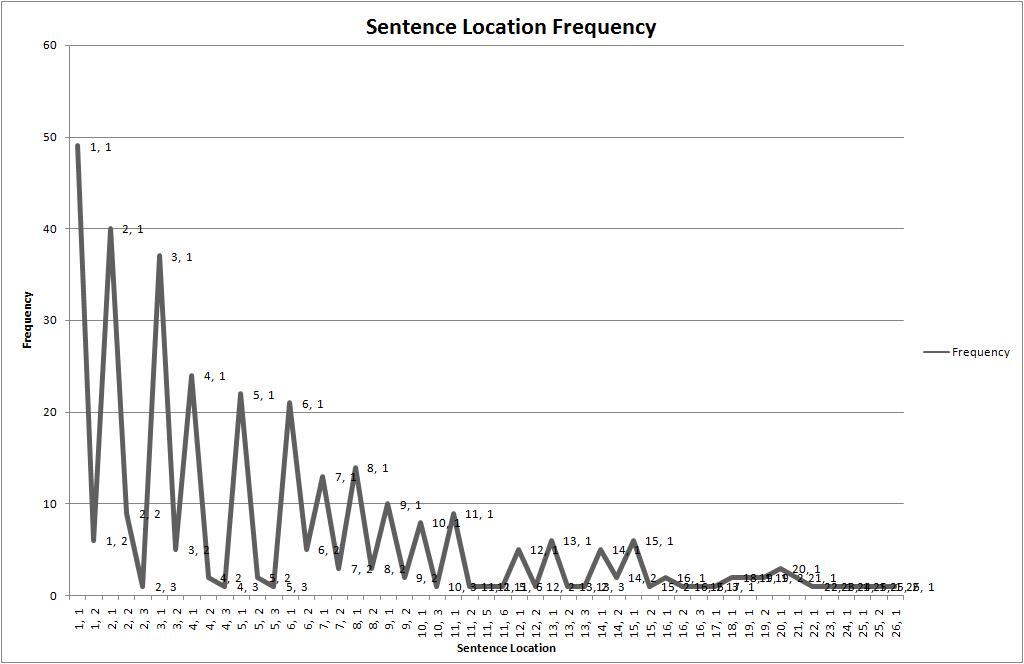
\includegraphics[scale=0.6]{/home/imran/Documents/myreport/Figure/sentloc}
 \caption{\singlespace Frequency distribution shows most frequent text locations contributing to extracts}
 \label{ch5:sentloc}
\end{figure}
\section{Determine frequent subunits(phrases) in the given text}
If the extraction mechanism only utilized the position hypothesis and assigned more importance to sentences at the top of the document, useful sentences at document depth
might have been lost. To retain such sentences frequent subunits(i.e. proper noun phrases) were extracted. Sentences were assigned weight as explained in section ~\ref{ch4:pnphrase}. 
The extraction mechanism ignores sentences with zero proper noun weight. It can be observed from the table ~\ref{ch5:tblpn} that the average weight assigned to sentences
of paragraph farther from the top of the document is more than the ones at the top, therefore sentences located at the end of paragraph or at the end of the entire 
document has a fair chance to contribute to extracts as long as the length specified to generate the extract allows. However, if the length specified to generate extracts
is reduced to very few words (e.g. 20 words for a document containing 300 or more words) the sentences containing frequent proper noun phrases are truncated.
It can also be easily observed from table ~\ref{ch5:tblpn} that choice of single best sentence is not straight forward, since sentences located at the end of document
might have more weight on the basis of proper noun phrases but at the same time less position based weight. 
\begin{table}[h]
\label{ch5:tblpn}
\caption{Frequency text locations of sample 50 extracts with average proper noun weight}
\begin{tabular}{|c|c|c|c|c|c|} 
\hline 
{\bf Location} & {\bf Frequency} & {\bf Avg PN Weight} & {\bf Location} & {\bf Frequency} & {\bf Avg PN Weight} \\ 
\hline 
     1,  1 &         49 &       1.39 &     11,  6 &          1 &       0.20 \\ 
\hline 
     1,  2 &          6 &       1.01 &     12,  1 &          5 &       0.60 \\ 
\hline 
     2,  1 &         40 &       1.52 &     12,  2 &          1 &       0.50 \\ 
\hline 
     2,  2 &          9 &       1.62 &     13,  1 &          6 &       0.31 \\ 
\hline 
     2,  3 &          1 &       0.50 &     13,  2 &          1 &       0.50 \\ 
\hline 
     3,  1 &         37 &       1.23 &     13,  3 &          1 &       0.17 \\ 
\hline 
     3,  2 &          5 &       1.71 &     14,  1 &          5 &       0.30 \\ 
\hline 
     4,  1 &         24 &       0.64 &     14,  2 &          2 &       0.58 \\ 
\hline 
     4,  2 &          2 &       0.28 &     15,  1 &          6 &       0.33 \\ 
\hline 
     4,  3 &          1 &       0.12 &     15,  2 &          1 &       0.10 \\ 
\hline 
     5,  1 &         22 &       1.09 &     16,  1 &          2 &       0.15 \\ 
\hline 
     5,  2 &          2 &       0.57 &     16,  2 &          1 &       0.10 \\ 
\hline 
     5,  3 &          1 &       0.33 &     16,  3 &          1 &       0.11 \\ 
\hline 
     6,  1 &         21 &       0.91 &     17,  1 &          1 &       0.10 \\ 
\hline 
     6,  2 &          5 &       0.26 &     18,  1 &          2 &       0.24 \\ 
\hline 
     7,  1 &         13 &       1.07 &     19,  1 &          2 &       0.12 \\ 
\hline 
     7,  2 &          3 &       0.21 &     19,  2 &          2 &       0.11 \\ 
\hline 
     8,  1 &         14 &       0.44 &     20,  1 &          3 &       0.40 \\ 
\hline 
     8,  2 &          3 &       0.23 &     21,  1 &          2 &       0.31 \\ 
\hline 
     9,  1 &         10 &       0.68 &     22,  1 &          1 &       1.00 \\ 
\hline 
     9,  2 &          2 &       0.32 &     23,  1 &          1 &       2.00 \\ 
\hline 
    10,  1 &          8 &       0.35 &     24,  1 &          1 &       1.00 \\ 
\hline 
    10,  3 &          1 &       0.50 &     25,  1 &          1 &       1.00 \\ 
\hline 
    11,  1 &          9 &       0.29 &     25,  2 &          1 &       1.00 \\ 
\hline 
    11,  2 &          1 &       0.50 &     26,  1 &          1 &       2.00 \\ 
\hline 
    11,  5 &          1 &       0.20 &          - &          - &          - \\ 
\hline 
\end{tabular}
\end{table}
\section{Parse extracted units containing frequent subunits for noun, verb, noun pattern}
Compression ratio(CR) is one of the quantitative measure used to test the output of summarizers, and sentence compression methods. Encapsulations for first sentences of
each news article in the sample data is evaluated for compression. Following formula is used to obtain compression ratio:-
\begin{displaymath}
  CR = (1 - (\frac{No\ of\ words\ in\ sentence}{No\ of\ words\ in\ encapsulation})) * 100
\end{displaymath}
Table ~\ref{ch5:CR} displays the classified results. It can be observed that compression ratio for 38 sentences out of 49 is above 50\%. However CR is not enough alone 
to evaluate result, encapsulation obtained should retain important information. In absence of standards to evaluate information retention, and time limitation
, an on-line survey consisting of thirteen sentences and their encapsulation was conducted. Thirteen participants scored encapsulated text for completeness of information.
The participants(graduate students of this institute) of the survey are proficient in English language.
From the result, listed under table ~\ref{ch5:Survey} it can be observed that there is general agreement on the encapsulation obtained by the system. Sentence number 13 
in table ~\ref{ch5:sentsur} is an example where encapsulation generated by the system would not completely represent the information. The reason for this degradation
is the contents of the sentence. If the contents of the sentence describe a law or an article of a constitution then dropping any of its phrases 
would result in unsatisfactory encapsulation.
\makeatletter
% http://www.texnik.de/floats/caption.phtml
% This does spacing around caption.
\setlength{\abovecaptionskip}{6pt}   % 0.5cm as an example
\setlength{\belowcaptionskip}{6pt}   % 0.5cm as an example
% This does justification (left) of caption.
\long\def\@makecaption#1#2{%
  \vskip\abovecaptionskip
  \sbox\@tempboxa{#1 #2}%
  \ifdim \wd\@tempboxa >\hsize
    #1: #2\par
  \else
    \global \@minipagefalse
    \hb@xt@\hsize{\box\@tempboxa\hfil}%
  \fi
  \vskip\belowcaptionskip}
\makeatother


 \begin{table}[h]
\label{ch5:CR}
\caption{CR obtained by encapsulation for 1st sentences of sample documents}
 \begin{tabular}{|c|c|}
 \hline
CR in \%age & No of sentences \\ \hline
Below 50 & 11 \\ \hline
50-60 & 6 \\ \hline
60-70 & 7 \\ \hline
70-80 & 13 \\ \hline
80-90 & 10 \\ \hline
Above 90 & 2 \\ \hline
 \end{tabular}
\end{table}



\begin{table}[h]
\label{ch5:Survey}
\caption{Information retention evaluated via on-line survey}
 \begin{tabular}{|c|c|c|c|c|}
 \hline
Sent No &  Strongly agree &  Agree &  Disagree &  Strongly disagree \\ \hline
1 &  2 &  9 &  2 &  0 \\ \hline
2 &  1 &  11 &  1 &  0 \\ \hline
3 &  2 &  7 &  3 &  1 \\ \hline
4 &  2 &  9 &  2 &  0 \\ \hline
5 &  3 &  5 &  5 &  0 \\ \hline
6 &  1 &  7 &  5 &  0 \\ \hline
7 &  1 &  7 &  5 &  0 \\ \hline
8 &  2 &  9 &  2 &  0 \\ \hline
9 &  1 &  10 &  2 &  0 \\ \hline
10 &  3 &  8 &  2 &  0 \\ \hline
11 &  0 &  7 &  6 &  0 \\ \hline
12 &  1 &  7 &  5 &  0 \\ \hline
13 &  2 &  6 &  4 &  1 \\ \hline
\end{tabular}
\end{table}


\begin{table}
\caption{Sentences used in survey with corresponding encapsulations}
\small{
\begin{longtable}{|p{16 cm}|}
\hline
{\bf Sentence 1:} \singlespace An explosion rocked the Royal Marines School of Music in a southeastern coastal town today, causing one building to collapse and killing eight people, officials said.   \\
{\bf Encap:} An explosion rocked the Royal Marines School  \\ \hline
{\bf Sentence 2: }\singlespace The communist world gets its first McDonald's next week, and some people here are wondering whether its American hamburgers will be as popular as the local fast-food treat, Pljeskavica. \\
{\bf Encap:} The communist world gets its first McDonald  \\ \hline
{\bf Sentence 3:} \singlespace   New treatments that stop a heart attack in its tracks may help victims to get out of the hospital more quickly than ever before, perhaps even three days after their attacks, a study published today concludes.  \\
{\bf Encap:}   New treatments that stop a heart attack  \\
\hline
{\bf Sentence 4:} \singlespace  A major earthquake rocked northern California Tuesday evening, collapsing part of the San Francisco Bay Bridge and shaking Candlestick Park and buildings up to 95 miles away.  \\
{\bf Encap:}   A major earthquake rocked northern California  \\
\hline
{\bf Sentence 5:} \singlespace  Thunderstorms wreaked havoc across the middle Mississippi Valley and the Southeast on Wednesday with lethal tornadoes, wind up to 100 mph and hail up to the size of baseballs.  \\
{\bf Encap:}   Thunderstorms wreaked havoc  \\ \hline
{\bf Sentence 6:} \singlespace  A strong earthquake hit the Himalayan kingdom of Nepal and parts of eastern India on Sunday morning, triggering landslides and collapsing buildings. \\
{\bf Encap:}   A strong earthquake hit the Himalayan kingdom  \\ \hline
{\bf Sentence 7:} \singlespace   Discovery's five astronauts returned Sunday for a second attempt to launch the shuttle with NASA's most valuable and celebrated payload, the \$1.5 billion Hubble Space Telescope.   \\
{\bf Encap:}   Discovery 's five astronauts returned Sunday  \\
\hline
{\bf Sentence 8:} \singlespace  Prime Minister Margaret Thatcher has weakened her position and kicked off the race to succeed her by saying she plans to step down after winning another term, opposition leaders and political observers said.  \\ 
{\bf Encap:}   Prime Minister Margaret Thatcher has weakened her position  \\ \hline
{\bf Sentence 9:} \singlespace  Defense Secretary-designate John Tower contradicted an earlier sworn statement when he told the Senate his work for a British firm involved no military matters, according to reports published Saturday.   \\
{\bf Encap:}   Defense Secretary-designate John Tower contradicted an earlier sworn statement  \\ \hline
{\bf Sentence 10:}  \singlespace Critic and novelist A.S. Byatt on Tuesday won the Booker Prize, Britain's most prestigious literary award, for her tale of two young scholars investigating the lives of a pair of imaginary Victorian poets.   \\
{\bf Encap:}   Critic and novelist A.S. Byatt Tuesday won the Booker Prize  \\ \hline
{\bf Sentence 11:}  \singlespace The blast occurred at at 8:26 a.m. in a lounge in the barracks near Deal, about 70 miles southeast of London, the Defense Ministry said.   \\
{\bf Encap:}   The blast occurred 8:26 a.m.  \\ \hline
{\bf Sentence 12:} \singlespace  The long-awaited opening of the restaurant on one of Belgrade's main downtown squares will take place March 24, the Yugoslav news agency Tanjug reported, and it will offer Big Macs, fries and the other specialities familiar to McDonald's customers in the West.   \\
{\bf Encap:}   The long-awaited opening the restaurant one Belgrade 's main downtown squares will take place  \\ \hline
{\bf Sentence 13:} \singlespace  Under a 1985 California law, insurers are required to offer earthquake insurance to homebuyers, but homebuyers are not required to buy the coverage.   \\
{\bf Encap:}   a 1985 California law insurers are required to offer earthquake insurance  \\ \hline
\end{longtable} }
\label{ch5:sentsur}
\end{table} 